
\documentclass{article}

\usepackage{graphicx}
\usepackage{amsmath}

\usepackage[margin=1in]{geometry}


\def\hwtitle{Computational Physics HW3}
\def\hwauthor{Ethan Rooney}
\def\hwdate{2020-02-12}

\usepackage{fancyhdr}
\lhead{\hwauthor}
\chead{\hwtitle}
\rhead{\hwdate}
\lfoot{\hwauthor}
\cfoot{}
\rfoot{\thepage}
\renewcommand{\footrulewidth}{0.4pt}
\pagestyle{fancy}

\author{\hwauthor}
\title{\hwtitle}
\date{\hwdate}

\begin{document}

\maketitle
\thispagestyle{fancy}

\section{Introduction}
 

\section{Results}

\bigskip
\noindent{\bf Question 1}
\medskip

Given Equation \ref{eq:1}: if we let $ r = 1 \text{AU}$ and $ \ddot{r} = a_c$ we can then use Equation \ref{eq:2} to find $ GM_{\cdot} = v^2r $. We know that $ v $ is the tangental velocity of the earth, which must travel $ 1 \text{AU} \times 2\pi \text{rad} $ per $ 1 \text{Year} $ we find $ GM_{\cdot} = 4\pi^2 \text{(AU^3)(Year^-2)} $.

\begin{equation} label{eq:1}
	\ddot{r} = \frac{GM_{\odot}}{r^2}\hat{r}
\end{equation}
\begin{equation} \label{eq:2}
	a_c = \frac{v^2}{r}
\end{equation}

\bigskip
\noindent{\bf Question 2}
\medskip

The Slope of a LogLog plot reveals power relationships. For the Left Integrator (The orange line in Figure \ref{fig:2}) the slope of the line can be found using Equation \ref{eq:3}. 

\begin{equation}\label{eq:3}
    \frac{\log(\epsilon_2)-\log(\epsilon_1)}{\log(bw_1)-\log(bw_2)}
\end{equation}

\begin{equation}\label{eq:4}
    \frac{\log(4.99917\times10^{-4})-\log(4.99999\times10^{-6})}{\log(10^{-3})-\log(10^{-5})} \simeq 1
\end{equation}{}

For $ bw_1 = 10^{-3}$ and $bw_2 = 10^{-5} $ we get equation \ref{eq:4} or a slope of 1. This indicates that $ \epsilon \propto 1/N$ where n is the number of bins.

For Plot see Figure \ref{fig:2}.

\begin{figure}[ht]\label{fig:2}
\begin{center}
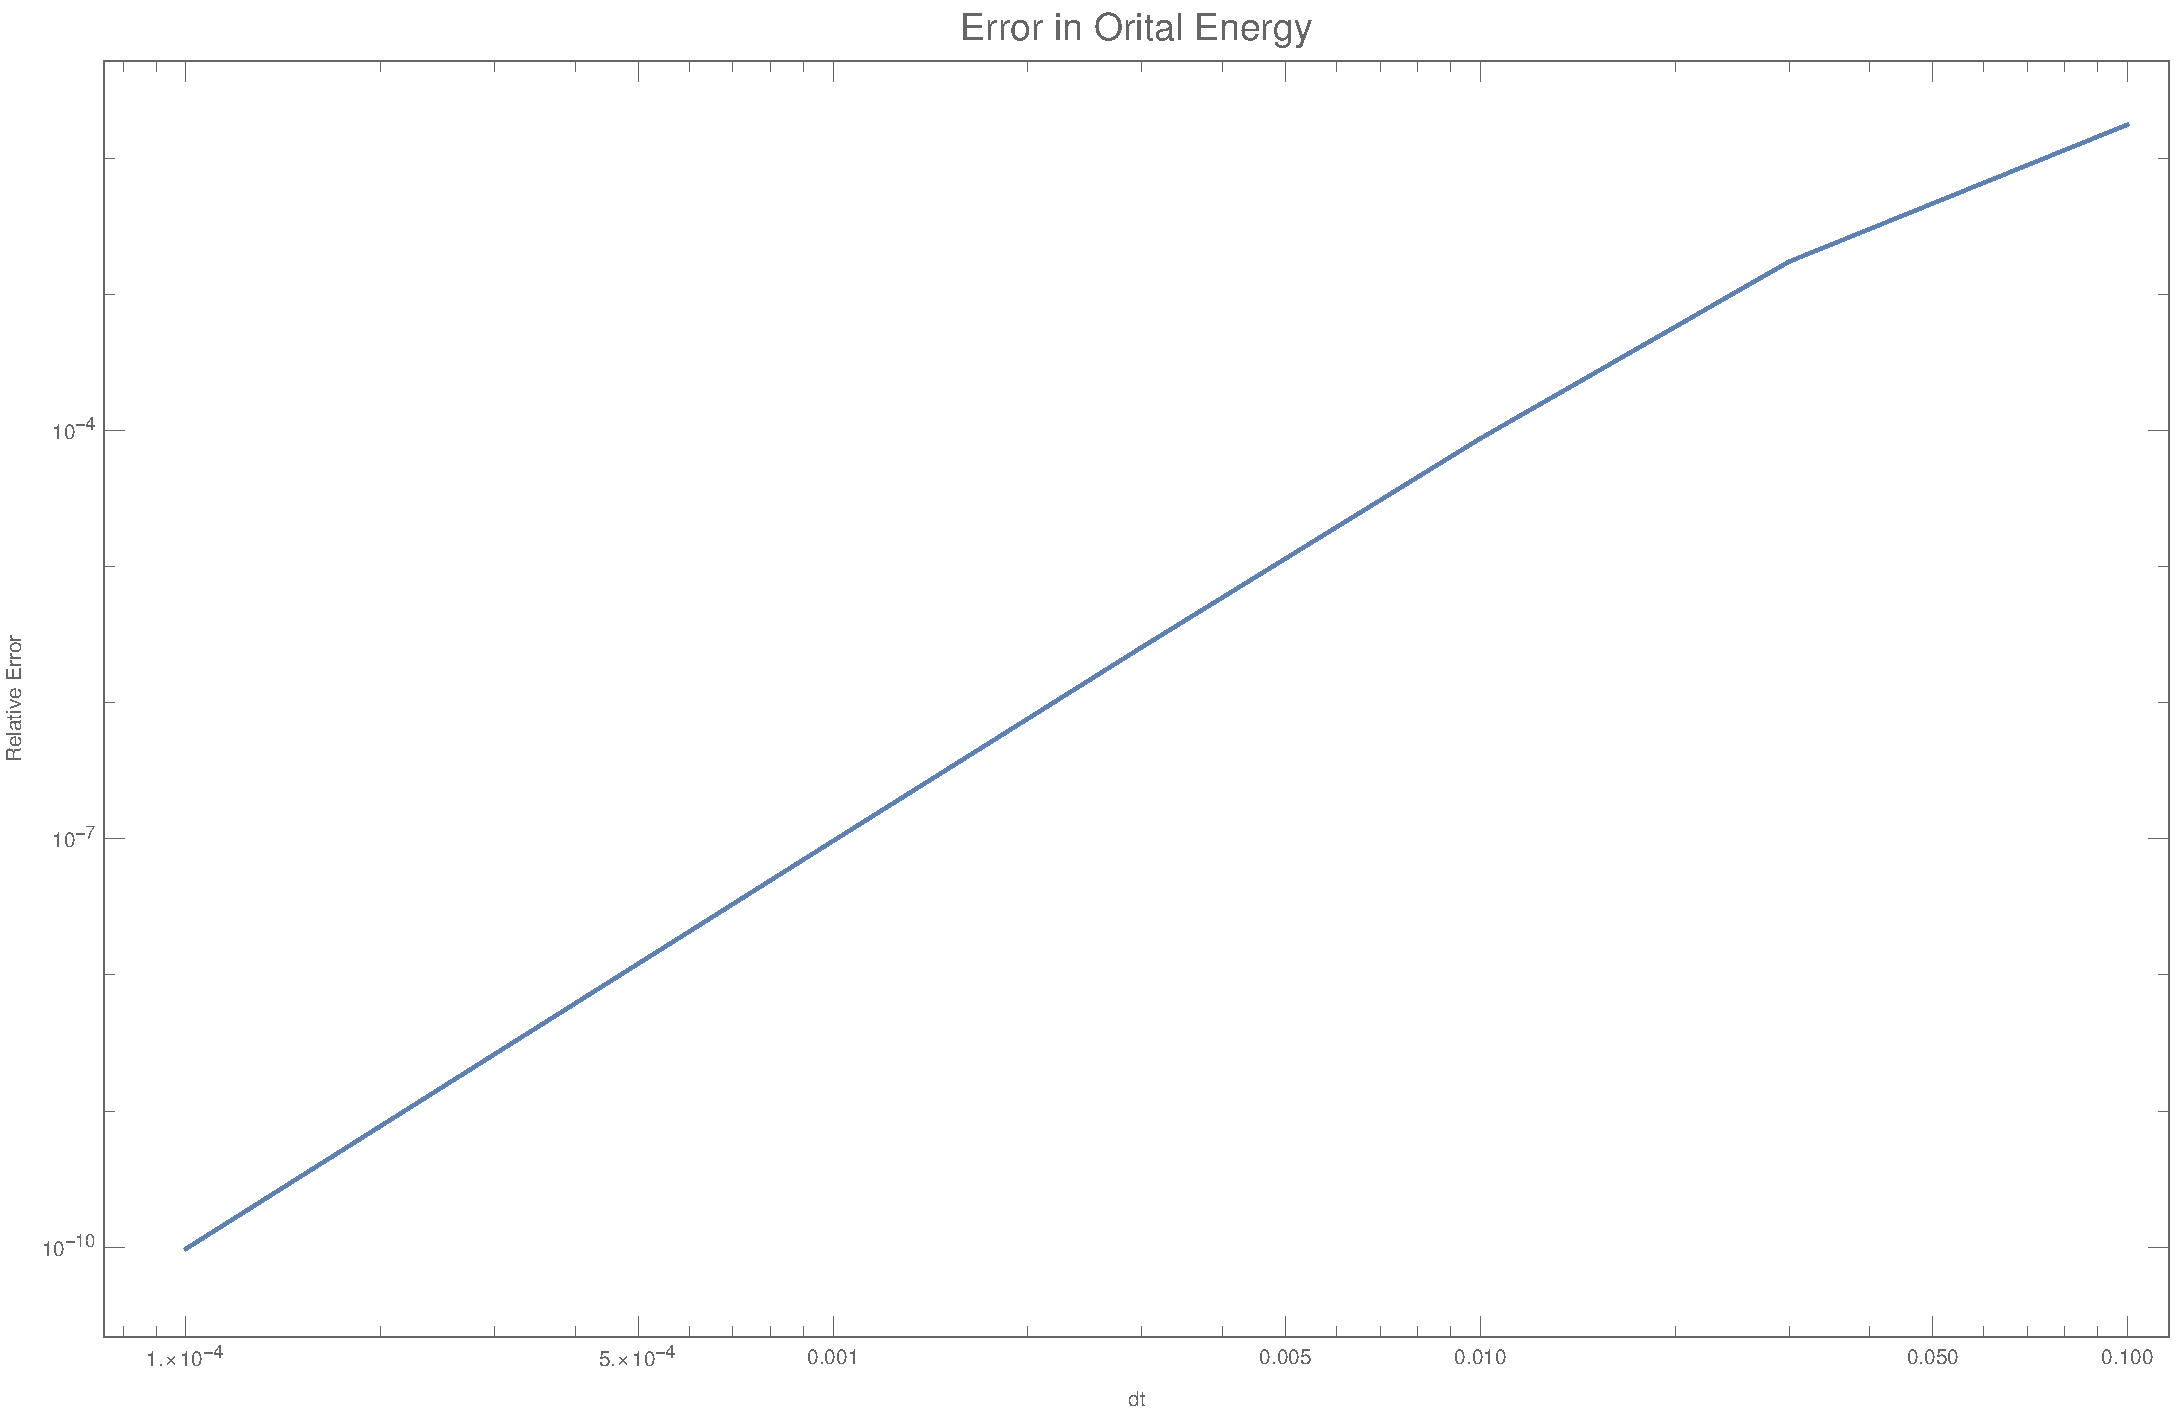
\includegraphics[width=0.5\textwidth]{error.pdf}
\end{center}
\caption{Effects of Bin Size vs the Relative error. The artifact near the bottom left of the Middle Integrator is due to the integrator meeting the precision of floating point numbers. Blue line represents Middle Integrator. Orange Represents Left Integrator}
\end{figure}

\bigskip
\noindent{\bf Question 3}
\medskip

Similar to the left hand integral for problem 2 we con compute the slope of the LogLog plot using Equation \ref{eq:3}. This gives the result seen in Equation \ref{eq:5}. Plot is located in Figure \ref{fig:2}.

\begin{equation}\label{eq:5}
    \frac{\log(4.16802\times10^{-12})-\log(4.16667\times10^{-8})}{\log(10^{-3})-\log(10^{-5})} \simeq 2
\end{equation}{}

This means that $\epsilon \propto \frac{1}{N^2}$. Meaning much fewer steps are required for  the function to converge.

\bigskip
\noindent{\bf Question 4}
\medskip

Given the following assumptions $ g = 9.81 \text{ ms}^{-2} $ and $ L=1\text{ m} $ for the small angle approximation we find Equation \ref{eq:6}. 

\begin{equation}\label{eq:6}
    \frac{\tau}{2} = \pi\sqrt{\frac{L}{g}} = 1.003s
\end{equation}

Using the Middle Integrator with $10^8$ bins for $ 15^\circ $ and $ 30^\circ $ we find $ \tau_{15}/2 = 1.020$ and $\tau_{30} = 1.076$

This gives us a relative error of $\epsilon_{15} = 1.6\times10^{-2}$ and $\epsilon_{30} = 7.3\times10^{-2}$ 

Therefore the $15^\circ$ clock will slow ~1460 seconds, and the $30^\circ$ clock will slow ~6290 seconds in a day.

\bigskip
\noindent{\bf Bonus}
\medskip

We see in Figure \ref{fig:3} the relative error for the Middle integrator.

Using Equation \ref{eq:3} we find the slope to be $\frac{1}{2}$. This indicates that $\epsilon \propto \frac{1}{\sqrt{N}}$.
I think the reason that the middle rule doesn't work as well is due to the rising and falling nature of the function. When the value only rises like in $e^x$ then the overestimate on the left half of the bin, approximately cancels the underestimate on the right.

When I tried to use my Left Integrator on the function I was returned with an \texttt{inf}. This is due to the $(cos(\theta)-cos(\theta_0)$ in the denominator. When using the left hand rule, the the first value attempted to compute will return $0$ causing the term to blowup.

\begin{figure}[ht]\label{fig:3}
\begin{center}
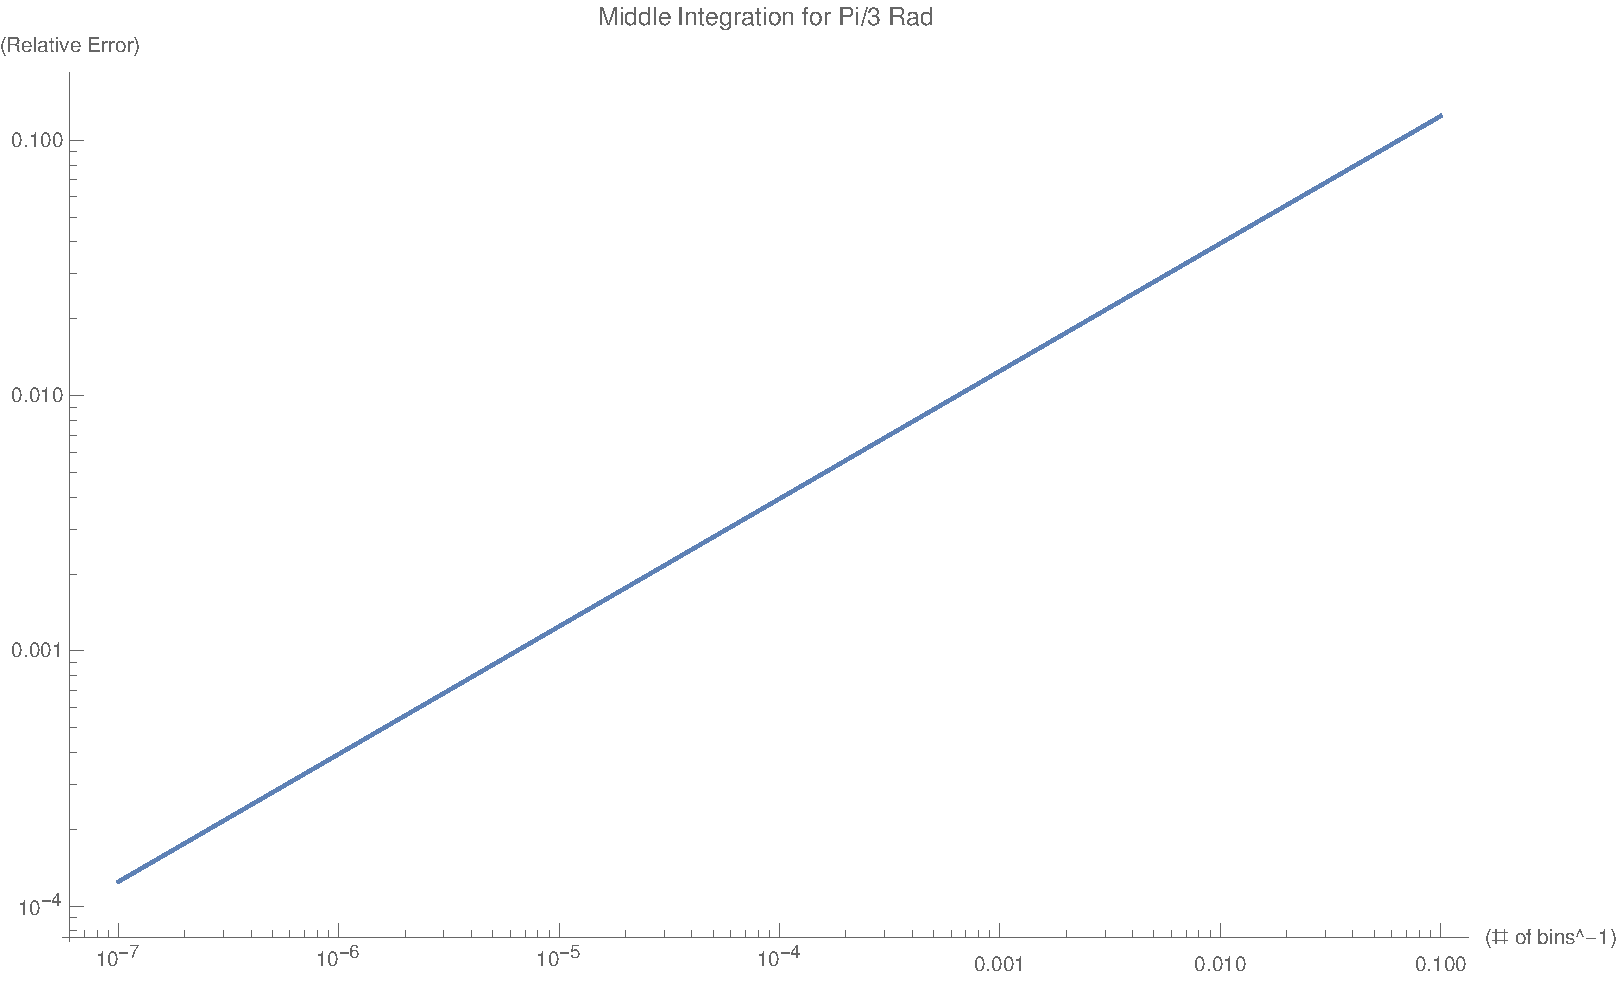
\includegraphics[width=0.5\textwidth]{pen30error.pdf}
\end{center}
\caption{Effects Bin Width vs the Relative Error for a Pendulum swinging at $30^\circ$}
\end{figure}

\section{Conclusions}

From these problems we can see that selection of integrator is contingent upon several criteria. First, computational time is important. Second, development time is also a factor. Third, the function to be approximated may work better with some integrator selections than others. Lastly, since type \texttt{double} has ~15 decimal digits of precision, care must be taken if precision beyond that is required.

As for trouble I encountered, Mathematica leaves much to be desired for a development environment. After a crash losing most of the work I developed on 04-02-2020, and another one the day this report was due, I will be looking for ways of interacting with the the Mathematica Kernel without having to use Mathematica.
\end{document}
